\chapter{Data availability}
\label{ap1}

\newpage

% %%%%%%%%%%%%%%%%%%%%%%%%%%%%%%%%%%%%%%%%%%%%
% \begin{figure}[t]
% %\footnotesize
% \begin{center}
% 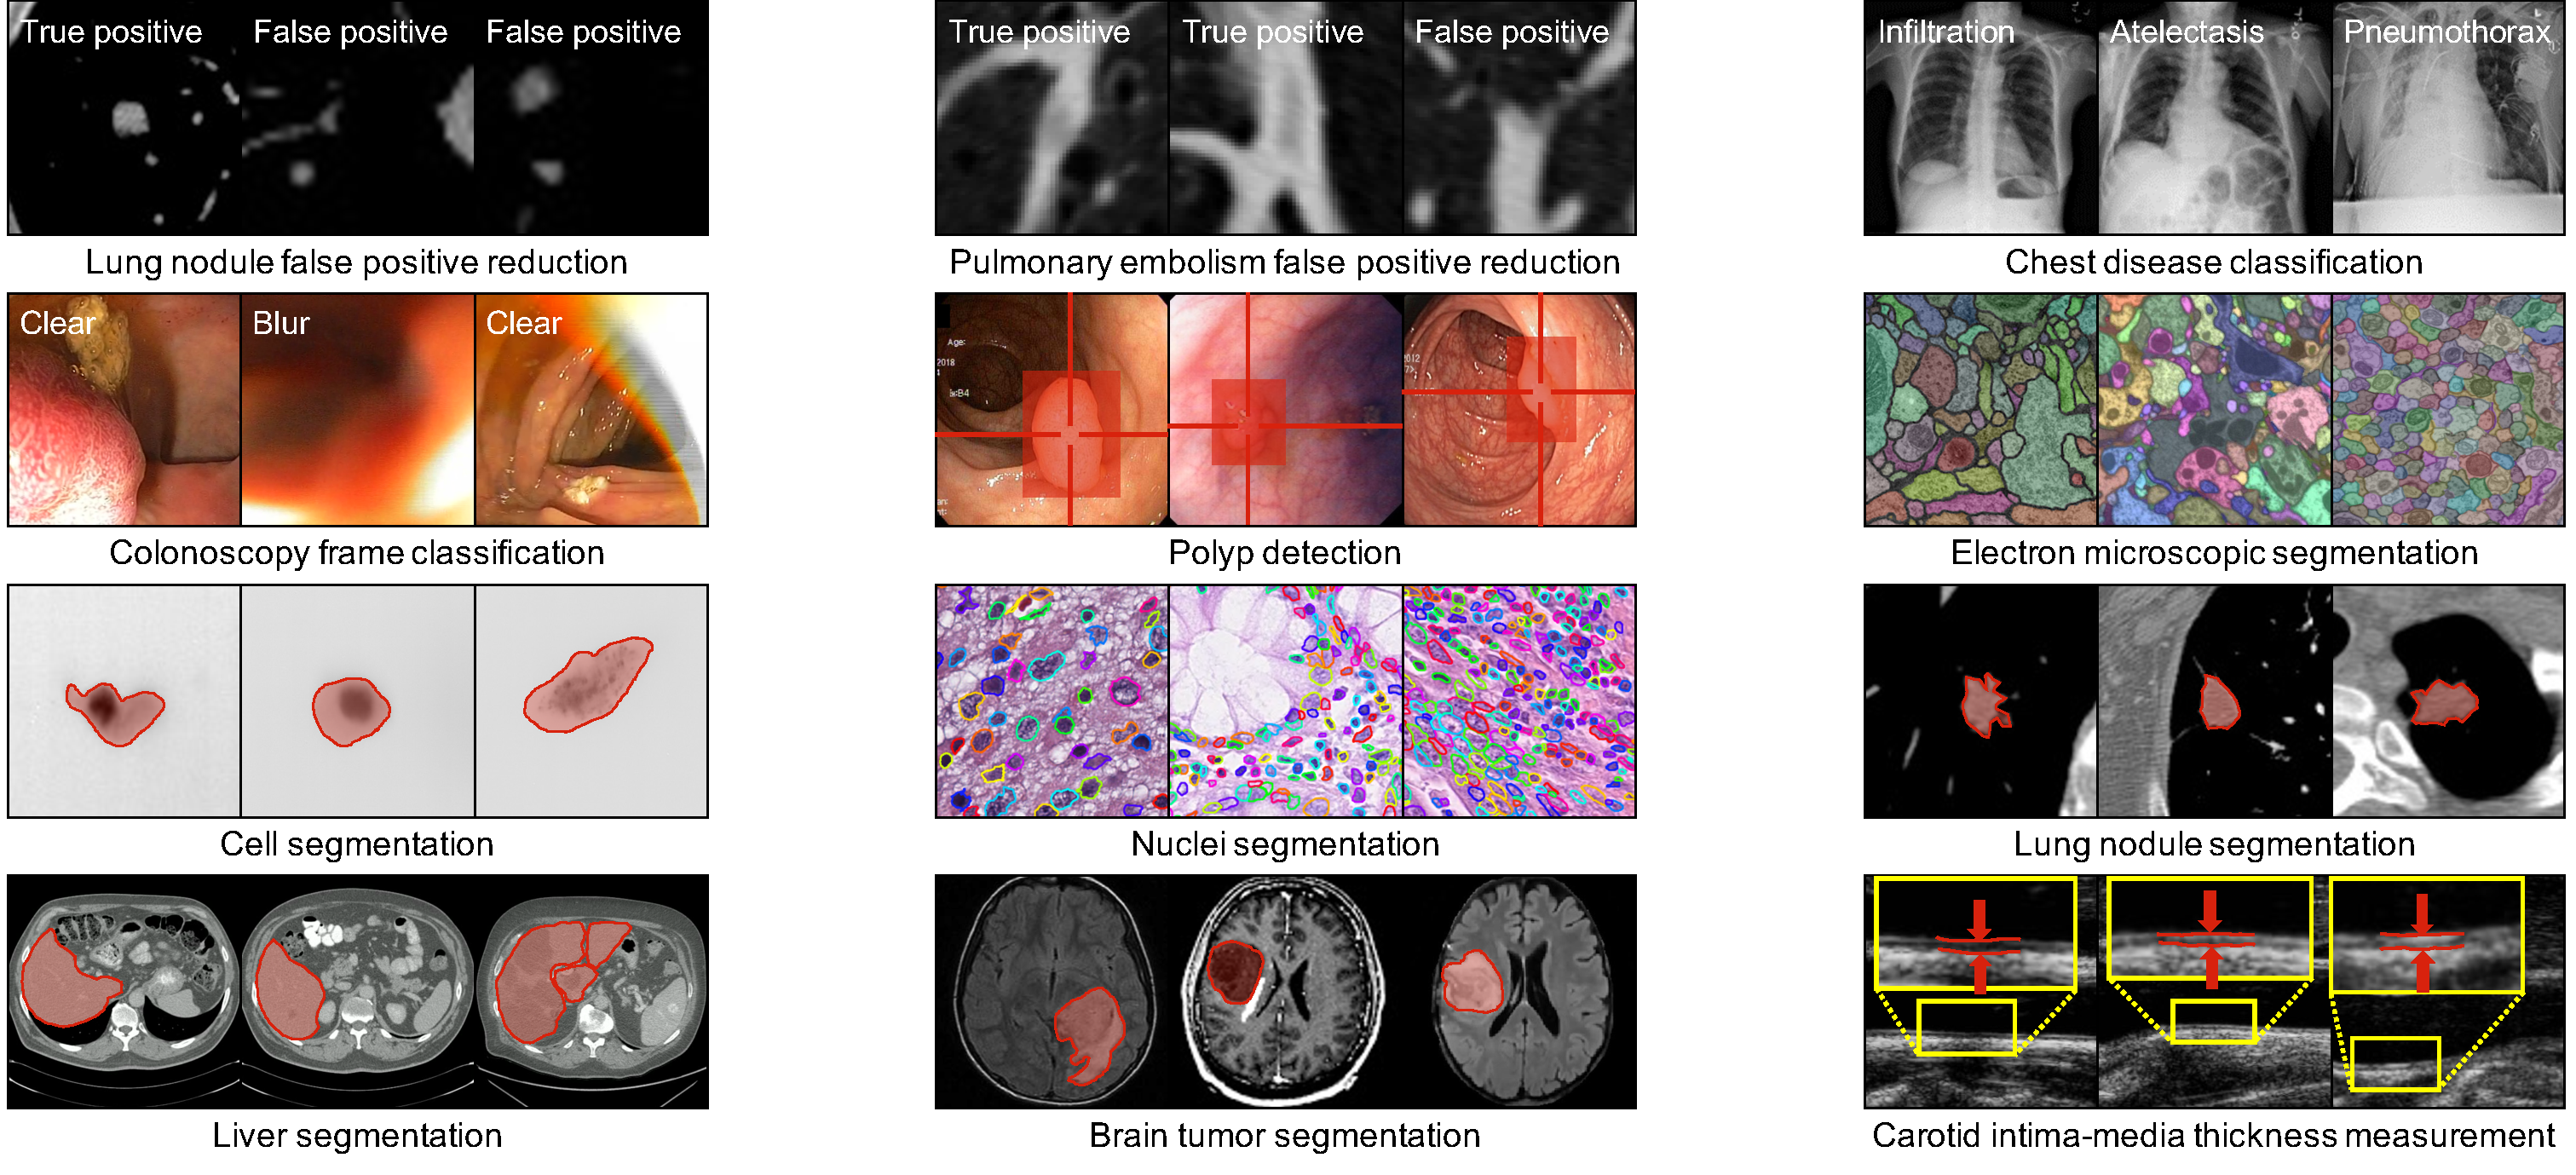
\includegraphics[width=1.0\linewidth]{Figures/AP1/fig_dataset_annotation.pdf}
% \end{center}
% \caption[Datasets and Annotations Used in This Dissertation]{Datasets and annotations used in this dissertation.}
% \label{ap1:fig:dataset_annotation}
% \end{figure}
% %%%%%%%%%%%%%%%%%%%%%%%%%%%%%%%%%%%%%%%%%%%%

%##############################################################################################
% \begin{landscape}
% \thispagestyle{empty}

\begin{sidewaysfigure}
\begin{center}
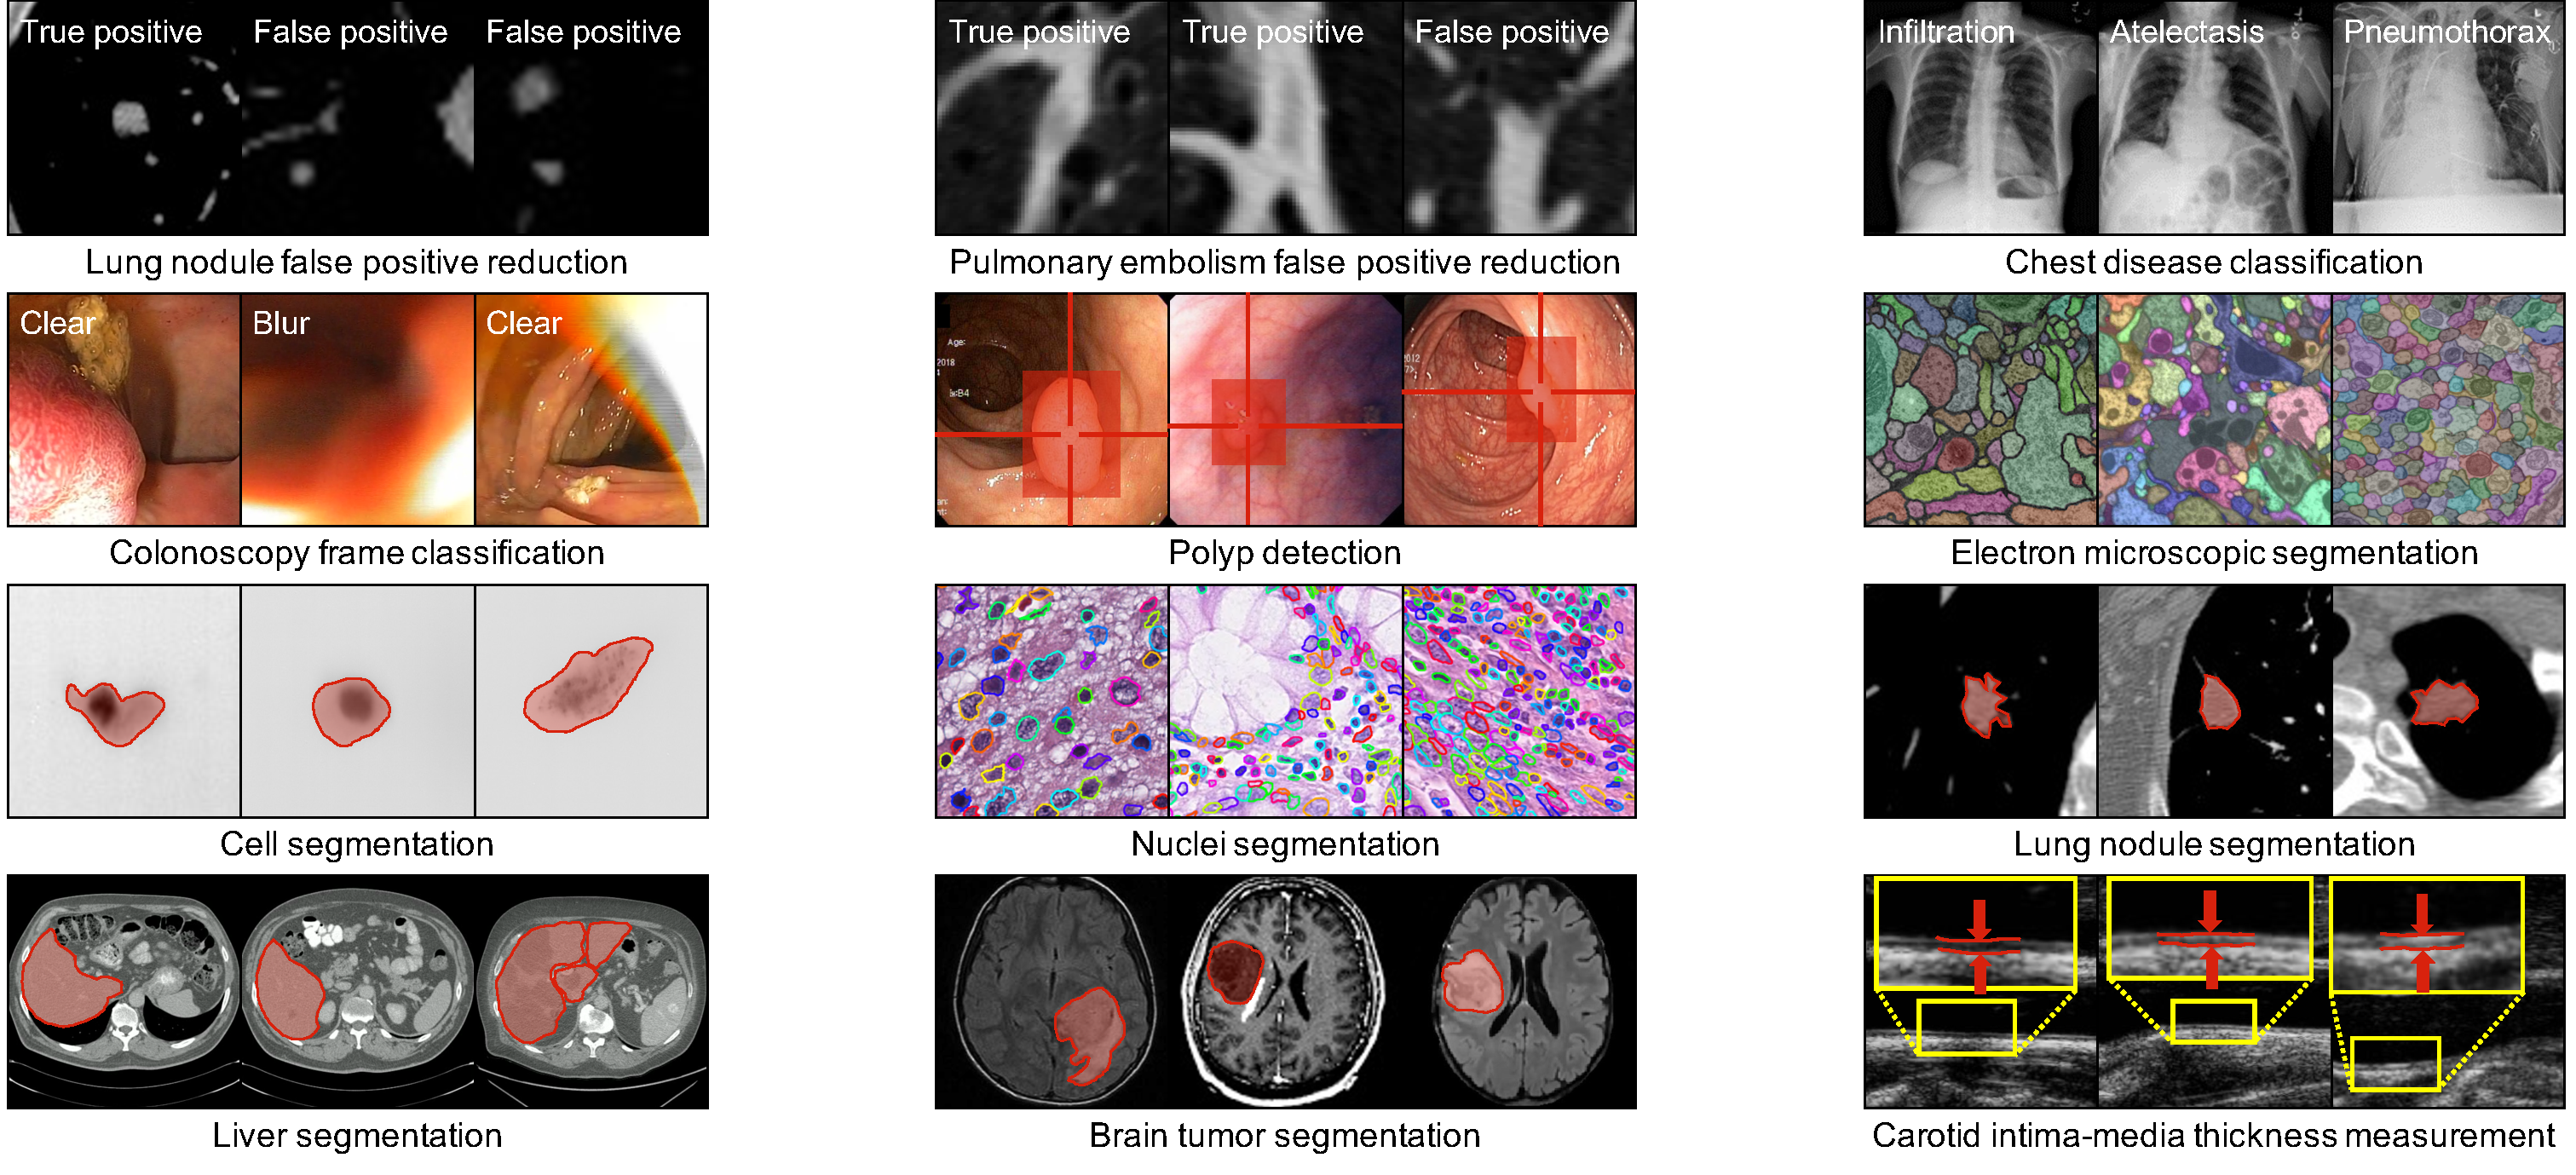
\includegraphics[width=1.0\linewidth]{Figures/AP1/fig_dataset_annotation.pdf}
\end{center}
\caption[Datasets and Annotations Used in This Dissertation]{Datasets and annotations used in this dissertation.}
\label{ap1:fig:dataset_annotation}
\end{sidewaysfigure}

% \fillandplacepagenumber
% \end{landscape}
%##############################################################################################


We summarizes the twelve medical imaging applications used in this dissertation, covering lesions/organs from most commonly used medical imaging modalities including microscopy, X-ray, computed tomography (CT), magnetic resonance imaging (MRI), and Ultrasound.

\section*{Lung Nodule False Positive Reduction}
\label{ap1:lung_nodule_classification}

The dataset is provided by LUNA~2016\footnote{\href{https://luna16.grand-challenge.org/}{https://luna16.grand-challenge.org/}}\citep{setio2017validation} and consists of 888 low-dose lung CTs with slice thickness less than 2.5mm. Patients are randomly assigned into a training set (445 cases), a validation set (178 cases), and a test set (265 cases). The dataset offers the annotations for a set of 5,510,166 candidate locations for the false positive reduction task, wherein true positives are labeled as ``1'' and false positives are labeled as ``0''. Following the prior works~\citep{setio2016pulmonary,sun2017automatic}, we evaluate performance via Area Under the Curve (AUC) score on classifying true positives and false positives.

\section*{Pulmonary Embolism False Positive Reduction}
\label{ap1:pulmonary_embolism_classification}

We utilize a database consisting of 121 computed tomography pulmonary angiography (CTPA) scans with a total of 326 emboli. 
Following the prior works~\citep{liang2007computer}, we utilize their PE candidate generator based on the toboggan algorithm, resulting in total of 687 true positives and 5,568 false positives. The dataset is then divided at the patient-level into a training set with 434 true positive PE candidates and 3,406 false positive PE candidates, and a test set with 253 true positive PE candidates and 2,162 false positive PE candidates. To conduct a fair comparison with the prior study~\citep{zhou2017fine,tajbakhsh2016convolutional,tajbakhsh2019computer}, we compute candidate-level AUC on classifying true positives and false positives.


\section*{Chest Disease Classification}
\label{ap1:chestxray}

This is a Chest X-ray dataset that we used to further validate the robustness of pre-trained weights on cross-disease, dataset, and modality situation.National Institutes of Health (NIH) provided Chest X-ray dataset\footnote{\href{https://www.kaggle.com/nih-chest-xrays/data}{https://www.kaggle.com/nih-chest-xrays/data}}\citep{wang2017chestx} consisting of frontal view chest X-ray PNG images with 8 thorax diseases:  Atelectasis, Cardiomegaly, Effusion, Infiltration, Mass, Nodule, Pneumonia, and Pneumothorax. As the dataset contains images with multi-labels, we used 8-dimensional label vector for each image. Furthermore, we normalize and shrink the image to 224$\times$224 resolution to match the input size of pre-trained models trained on ImageNet. The dataset is divided at the patient-level into a training set with 43,976 images of 21,563 patients, validation set with 9,125 images of 4,621 patients, and test set with 9,171 images of 4,621 patients.


\section*{Colonoscopy Frame Classification}
\label{ap1:colonoscopy_frame_classification}

Image quality assessment in colonoscopy can be viewed as an image classification task whereby an input image is labeled as either \textit{clear} or \textit{blur}. 
One way to measure the quality of a colonoscopy procedure is to monitor the quality of the captured images. Such quality assessment can be used during live procedures to limit low-quality examinations or, in a post-processing setting, for quality monitoring purposes.
In this application, colonoscopy frames are regarded as \textit{candidates}, since the labels (clear or blur) are associated with frames as illustrated in \figurename~\ref{ap1:fig:dataset_annotation}.  In total, there are 4,000 colonoscopy candidates from 6 complete colonoscopy videos. A trained expert then manually labeled the collected images as clear or blur (line 11 in Alg.~\ref{ch3:alg:ACFT}). A gastroenterologist further reviewed the labeled images for corrections. The labeled frames are separated at the video level into training and test sets, each containing approximately 2,000 colonoscopy frames. For data augmentation, we extracted 21 patches from each frame as shown in \figurename~\ref{ap1:fig:dataset_annotation}(d).


\section*{Polyp Detection}
\label{ap1:polyp_detection}

Polyps, as shown in \figurename~\ref{ap1:fig:dataset_annotation}, can present themselves in the colonoscopy with substantial variations in color, shape, and size. The variable appearance of polyps can often lead to misdetection, particularly during long and back-to-back colonoscopy procedures where fatigue negatively affects the performance of colonoscopists. Computer-aided polyp detection may enhance optical colonoscopy screening accuracy by reducing polyp misdetection. 
In this application, each polyp detection is regarded as a \textit{candidate}.
The dataset contains 38 patients with one video each. The training dataset is composed of 21 videos (11 with polyps and 10 without polyps), while the testing dataset is composed of 17 videos (8 videos with polyps and 9 videos without polyps). At the video level, the candidates are divided into the training dataset (16,300 candidates) and test dataset (11,950 candidates). At each polyp candidate location with the given bounding box, we performed data augmentation by a factor $f\in \{1.0,1.2,1.5\}$. At each scale, we extracted patches after the candidate is translated by 10 percent of the resized bounding box in vertical and horizontal directions. We further rotated each resulting patch 8 times by mirroring and flipping. The patches generated by data augmentation belong to the same candidate. Each candidate contains 24 patches.


\section*{Electron Microscopic Segmentation}
\label{ap1:electron_microscopic_segmentation}

The dataset is provided by the EM segmentation challenge\footnote{\href{http://brainiac2.mit.edu/isbi_challenge/home}{http://brainiac2.mit.edu/isbi\_challenge/home}}\citep{cardona2010integrated} as a part of ISBI 2012. The dataset consists of 30 images (512$\times$512 pixels) from serial section transmission electron microscopy of the Drosophila firt instar larva ventral nerve cord (VNC). Referring to the example in~\figurename~\ref{ap1:fig:dataset_annotation}, each image comes with a corresponding fully annotated ground truth segmentation map for cells (white) and membranes (black). The labeled images are split into training (24 images), validation (3 images), and test (3 images) datasets. 
Both training and inference are done based on 96$\times$96 patches, which are chosen to overlap by half of the patch size via sliding windows. Specifically, during the inference, we aggregate predictions across patches by voting in the overlapping areas.


\section*{Cell Segmentation}
\label{ap1:cell_segmentation}

The dataset is acquired with a Cell-CT imaging system~\citep{meyer2015cell}. Two trained experts manually segment the collected images, so each image in the dataset comes with two binary cell masks. For our experiments, we select a subset of 354 images that have the highest level of agreement between the two expert annotators. The selected images are then split into training (212 images), validation (70 images), and test (72 images) subsets.

\section*{Nuclei Segmentation}
\label{ap1:nuclei_segmentation}

The dataset is provided by the Data Science Bowl 2018 segmentation challenge\footnote{\href{https://www.kaggle.com/c/data-science-bowl-2018}{https://www.kaggle.com/c/data-science-bowl-2018}} and consists of 670 segmented nuclei images from different modalities (brightfield vs. fluorescence). This is the only dataset used in this work with instance-level annotation where each nucleolus is marked in a different color. Images are randomly assigned into a training set (50\%), a validation set (20\%), and a test set (30\%). We then use a sliding window mechanism to extract 96$\times$96 patches from the images, with 32-pixel stride for training and validating model, and with 1-pixel stride for testing. 


\section*{Lung Nodule Segmentation}
\label{ap1:lung_nodule_segmentation}

The dataset is provided by the Lung Image Database Consortium image collection (LIDC-IDRI)\footnote{\href{https://wiki.cancerimagingarchive.net/display/Public/LIDC-IDRI}{https://wiki.cancerimagingarchive.net/display/Public/LIDC-IDRI}}\citep{armato2011lung} and consists of 1,018 cases collected by seven academic centers and eight medical imaging companies. The cases were split into training (510), validation (100), and test (408) sets. Each case is a 3D CT scan and the nodules have been marked as volumetric binary masks. We have re-sampled the volumes to 1-1-1 spacing and then extracted a $64\times 64\times 32$ crop around each nodule. These 3D crops are used for model training and evaluation. As in prior works~\citep{aresta2019iw,tang2019nodulenet,zhou2018unet++}, we adopt Intersection over Union (IoU) and Dice coefficient scores to evaluate performance. Note that for this particular application, we calculate mean of the IoUs at thresholds ranging from 0.5 to 0.95 with a step size of 0.05.

\section*{Liver Segmentation}
\label{ap1:liver_segmentation}

The dataset is provided by MICCAI 2017 LiTS Challenge\footnote{\href{https://competitions.codalab.org/competitions/17094}{https://competitions.codalab.org/competitions/17094}} and consists of 130 labeled CT scans, which we split into training (100 patients), validation (15 patients), and test (15 patients) subsets. The ground truth segmentation provides two different labels: liver and lesion. For our experiments, we only consider liver as positive class and others as negative class and evaluate segmentation performance using Intersection over Union (IoU) and Dice coefficient scores.

\section*{Brain Tumor Segmentation}
\label{ap1:brain_tumor_segmentation}

The dataset is provided by BraTS~2013~\citep{kistler2013virtual} and BraTS~2018~\citep{menze2015multimodal,bakas2018identifying} challenges\footnote{\href{http://braintumorsegmentation.org/}{http://braintumorsegmentation.org/}}. For experiments in Chapter~\ref{ch3}, the models are trained using 20 High-grade (HG) and 10 Low-grade (LG) with Flair, T1, T1c, and T2 scans of MR images from all patients in BraTS~2013, resulting in a total of 66,348 slices. We further pre-process the dataset by re-scaling the slices to 256$\times$256. Finally, the  30 patients available in the dataset are randomly assigned into five folds, each having images from six patients. We then randomly assign these five folds into a training set (3-fold), a validation set (1-fold), and a test set (1-fold). The ground truth segmentation have four different labels: necrosis, edema, non-enhancing tumor, and enhancing tumor. Following the BraTS-2013, the ``complete'' evaluation is done by considering all four labels as positive class and others as negative class. For experiments in Chapter~\ref{ch4}, we utilize BraTS~2018, which consists of 285 patients (210 HGG and 75 LGG), each with four 3D MRI modalities (T1, T1c, T2, and Flair) rigidly aligned. We adopt 3-fold cross validation, in which two folds (190 patients) are for training and one fold (95 patients) for test. Annotations include background (label 0) and three tumor subregions: GD-enhancing tumor (label 4), the peritumoral edema (label 2), and the necrotic and non-enhancing tumor core (label 1). We consider those with label 0 as negatives and others as positives and evaluate segmentation performance using Intersection over Union (IoU) and Dice coefficient scores.


\section*{Carotid Intima-media Thickness Measurement}
\label{ap1:cimt_measurement}

Cardiovascular disease (CVD) is the leading cause of death in the United States: every 40 seconds one American dies of CVD; nearly one-half of these deaths occur suddenly and one-third of them occur in patients younger than 65 years, but CVD is preventable. To prevent CVD, the key is to identify at-risk individuals, so that scientifically proven and efficacious preventive care can be prescribed appropriately. Carotid intima-media thickness (CIMT) measurement, a noninvasive ultrasonography method, has proven to be clinically valuable for predicting individual CVD risk~\citep{stein2008use,gepner2015comparison}. It quantifies subclinical atherosclerosis, adds predictive value to traditional risk factors (\eg the Framingham risk score), and has several advantages over computed tomography (CT) coronary artery calcium score: safer (no radiation exposure), more sensitive in a young population, and more accessible to the primary care setting.  However, as illustrated by~\citet{shin2016automating} in their \figurename~1, interpretation of CIMT videos involves three manual operations, which are not only tedious and laborious but also subjective to large interoperator variability if guidelines are not properly followed, hindering the widespread utilization of CIMT in clinical practice. 

We focus on the two most important tasks: ROI localization and thickness measurement. We utilize 23 patients from UFL MCAEL CIMT research database~\citep{hurst2010incidence}. Each patient has four videos (two on each side)~\citep{stein2008use}, resulting in a total of 92 CIMT videos with 8,021 frames. Each video covers at least 3 cardiac cycles and thus a minimum of 3 EUFs. We randomly divide the CIMT videos at patient level into training, validation, and test sets (no overlaps). The training set contains 44 CIMT videos of 11 patients with a total of 4,070 frames, the validation set contains  4 videos of 1 patient with 386 frames, and the test set contains 44 CIMT videos of 11 patients with 3,565 frames. From the perspective of active learning, the training set is initially the ``unlabeled pool" for active selection; when an \texttt{AU} is selected, its label will be provided. The fined-tuned CNN from each iteration is always evaluated with the test set, so that we can monitor the performance enhancement across \texttt{AU}s. Please note that we do not need many patients as we have many CIMT frames for each patient and we can generate a large number of patches for training deep models in each experiment. For example, in our ROI localization experiments, one \texttt{AU} practically provides 1,715 labeled patches (297 as {\em background}, 709 as {\em bulb} and 709 as {\em ROI}). Random translation and flipping data augmentation were applied when training the models.